% !TEX root = ../main.tex
\chapter{Hankel Alternative View of Koopman (HAVOK)}\label{ch:havok}
\begin{paracol}{2}

\begin{sources}
\begin{tabularx}{\linewidth}{@{}V l L@{}}
\toprule
\textbf{Video} & \textbf{Length} & \textbf{Content}\\
\midrule
\seg{8}{1}{V8.1 Hankel Alternative View of Koopman (HAVOK) Analysis [FULL]} & 47:07 & Chaos; Koopman invariant subspaces; Hankel matrix and eigen time-delay coordinates; the Koopman reading of the Hankel matrix; the forced linear model; intermittent forcing and lobe switching; Perron--Frobenius almost-invariant sets; magnetic field and measles; the structure of the model, integer coefficients.\\
\seg{8}{2}{V8.2 Hankel Alternative View of Koopman (HAVOK) Analysis [SHORT]} & 22:41 & The same method in short; choice of $r$ by the optimal hard threshold; only what is new is cited.\\
\seg{8}{3}{V8.3 Magnetic field reversal and Measles outbreaks: HAVOK models of chaos} & 9:39 & The two real-world examples in more detail.\\
\seg{8}{4}{V8.4 Linear model for chaotic Lorenz system [HAVOK]} & 5:27 & The sparse antisymmetric structure of $A$; the integer-coefficient model.\\
\bottomrule
\end{tabularx}

\smallskip
\textbf{Transcripts} \file{materials/transcripts/C08-V0*.txt}.
\textbf{Book} Sec.~7.5 (``Time-delay coordinates'', HAVOK).
\textbf{Paper} S.~L.~Brunton, B.~W.~Brunton, J.~L.~Proctor, E.~Kaiser, J.~N.~Kutz, \emph{Chaos as an intermittently forced
linear system}, Nat.\ Commun.\ 8 (2017) 19.
\textbf{Code} \file{code/ch08_havok.py} (original Matlab code: faculty.washington.edu/sbrunton/HAVOK.zip).
The SHORT video repeats the FULL one: it is cited only where it adds something.
\end{sources}

\section*{Motivation}
The last chapter brings together everything: delay coordinates (\cref{sec:si-extensions}), Koopman invariant subspaces
(\cref{ch:koopmancontrol}), DMD/SINDy regression (\cref{ch:dmd,ch:sindy}) and chaos (\cref{ch:fundamentals}). The result:
a chaotic system, observed through a single time series, is well described as a \emph{linear} system driven by an
\emph{intermittent forcing}, and the forcing announces rare nonlinear events, such as lobe switching in Lorenz, before
they happen \ts{8}{1}{0:02}\ts{8}{1}{0:22}. \Cref{prop:kc-topology} said that no finite linear model containing the state can
reproduce several fixed points; HAVOK sidesteps it by letting a forcing carry the essential nonlinearity.

% ------------------------------------------------------------------
\section{Chaos and the Koopman view}\label{sec:hv-chaos}

Chaotic systems are everywhere: climate, turbulence, the stock market, epidemics, planetary motion \ts{8}{1}{0:44}. Linear
systems have the full toolbox of prediction, estimation and control; nonlinear ones have multiple fixed points (the double
well), periodic orbits, and with more nonlinearity chaos \ts{8}{1}{2:25}\ts{8}{1}{2:46}\ts{8}{1}{3:07}. Two double pendulums
released side by side from nearly the same state stay synchronized for a while, then do completely different acrobatics
\ts{8}{1}{3:48}\ts{8}{1}{4:09}. A cube of initial conditions in Lorenz is stretched and folded ``like taffy'' over the
attractor \ts{8}{1}{4:50}\ts{8}{1}{5:11}\ts{8}{1}{5:32}.

\begin{intuition}[Chaos is not randomness]
The smeared cube is not random: it forms structured, coherent patterns. Chaos balances order and structure against
uncertainty amplification in forward time \ts{8}{1}{5:52}\ts{8}{1}{6:12}\ts{8}{2}{1:05}. That structure is what HAVOK
exploits.
\end{intuition}

Koopman recap: propagate measurements $g(\vb x)$ linearly, at the price of infinite dimension; a Koopman-invariant subspace
gives a matrix, but such subspaces are hard to find \ts{8}{1}{6:53}\ts{8}{1}{7:55}\ts{8}{1}{9:17}\ts{8}{1}{9:58}. HAVOK is an
alternative way to get one for chaotic systems; the acronym ``goes nicely with chaos'' \ts{8}{1}{10:19}\ts{8}{1}{10:41}.

% ------------------------------------------------------------------
\section{Delay coordinates and the Koopman reading of the Hankel matrix}\label{sec:hv-hankel}

\paragraph{Embedding.} Measure only $x(t)$ of Lorenz: it sits on one lobe, switches to the other, unpredictably
\ts{8}{1}{11:23}\ts{8}{1}{11:43}. Build the Hankel matrix \eqref{eq:si-hankel} from time-shifted copies of the series
\ts{8}{1}{12:04}\ts{8}{1}{12:24} and take its SVD, $H=U\Sigma V^*$. The columns of $U$ and $V$ are ordered by singular value: the
first ones are the time series most self-similar to the measurement \ts{8}{1}{12:45}\ts{8}{1}{13:06}\ts{8}{1}{13:27}. The idea is old:
the eigensystem realization algorithm (1985), singular spectrum analysis in climate, and the recent nonlinear Laplacian
spectral analysis of Giannakis and Majda \ts{8}{1}{13:48}\ts{8}{1}{14:09}. Plotting $(v_1,v_2,v_3)$ gives an attractor
diffeomorphic to Lorenz's, by Takens' theorem (\cref{thm:si-takens}); $x$ is a good measurement, $z$ would be a bad one
(it cannot distinguish the two lobes, by the symmetry $(x,y,z)\mapsto(-x,-y,z)$) \ts{8}{1}{14:29}\ts{8}{1}{14:50}\ts{8}{1}{15:11}.

\paragraph{The Koopman reading.} Since $x(t_{k+1})=\K x(t_k)$, the Hankel matrix is a Krylov sequence of the Koopman operator
\ts{8}{1}{15:53}\ts{8}{1}{16:13}\ts{8}{1}{16:33}:
\begin{equation}\label{eq:hv-krylov}
  H=\begin{bmatrix}x(t_1)&x(t_2)&\cdots\\ x(t_2)&x(t_3)&\cdots\\ \vdots&&\end{bmatrix}
   =\begin{bmatrix}x(t_1)&\K x(t_1)&\K^2x(t_1)&\cdots\\ \K x(t_1)&\K^2x(t_1)&\cdots\\ \vdots&&\end{bmatrix}.
\end{equation}
Thousands of columns, but numerically of low rank: for Lorenz the first $r=15$ columns of $U$ express every column of $H$ to
almost machine precision \ts{8}{1}{16:54}\ts{8}{1}{17:15}\ts{8}{1}{17:37}. Each column is $\K$ applied to the previous one, so the
span of the leading columns of $U$ is (approximately) \emph{Koopman invariant}: a data-driven invariant measurement subspace of
eigen time-delay coordinates \ts{8}{1}{17:58}\ts{8}{2}{12:07}\ts{8}{2}{12:27}. In the SHORT video $r=15$ is chosen with the optimal
hard threshold of Gavish and Donoho \ts{8}{2}{18:21}.

\begin{remark}[Why chaos helps]
This works best for chaotic systems: the trajectory never returns exactly and densely explores the attractor, never stuck at
a fixed point or a periodic orbit, so one global model for the attractor makes sense, and more data make the linear dependence
better \ts{8}{1}{18:19}\ts{8}{1}{18:39}\ts{8}{1}{19:00}. It holds for data on the attractor, not for every initial condition
\ts{8}{2}{12:27}.
\end{remark}

\begin{secondary}[Singular values of the Lorenz Hankel matrix]
In \file{ch08_havok.py} ($dt=0.001$, $q=100$ delays, $t\in[0,200]$) the singular values relative to the first are $1$,
$0.15$, $0.02$, $2.4\times10^{-3}$, $2.8\times10^{-4}$, $3\times10^{-5}$, \dots: a geometric decay by roughly a factor 8 each.
For a short window ($q\,dt=0.1$) the delay vector is essentially a Taylor expansion of $x(t)$ around the window, which is why
the modes $u_k$ look like Legendre polynomials (see \cref{sec:hv-structure}) and why the singular values decay geometrically.
\end{secondary}

% ------------------------------------------------------------------
\section{Chaos as an intermittently forced linear system}\label{sec:hv-model}

Regress the time derivatives of the eigen time-delay coordinates on the coordinates themselves, as in DMD or SINDy but on
$\vb v=(v_1,\dots,v_r)$ \ts{8}{1}{19:41}\ts{8}{1}{20:01}\ts{8}{1}{20:22}. The first $r-1$ equations fit very well; the last one, for
$v_r$, fits terribly, even with nonlinear terms \ts{8}{1}{20:43}\ts{8}{1}{21:05}\ts{8}{1}{21:25}\ts{8}{1}{21:46}. So treat $v_r$ as an
external input \ts{8}{1}{22:06}:
\begin{equation}\label{eq:hv-model}
  \frac{\mathrm d}{\mathrm dt}\begin{bmatrix}v_1\\\vdots\\v_{r-1}\end{bmatrix}=A\begin{bmatrix}v_1\\\vdots\\v_{r-1}\end{bmatrix}+B\,v_r(t).
\end{equation}

\begin{definition}[New concepts: HAVOK]\label{def:hv}
The \textbf{Hankel alternative view of Koopman} (HAVOK) model of a scalar time series is \eqref{eq:hv-model}: a linear
system in the first $r-1$ eigen time-delay coordinates, forced by the $r$-th, obtained by least-squares regression. A
\textbf{Hankel} matrix (after Hermann Hankel, 1839--1873) is constant along its anti-diagonals.
\end{definition}

\paragraph{What the model does.} Fed with the measured forcing $v_r$ (in red), the linear model reproduces the dynamics (blue
over the white data) and the attractor; and the forcing bursts exactly when the trajectory switches lobes \ts{8}{1}{22:48}\ts{8}{1}{23:08}\ts{8}{1}{23:29}\ts{8}{1}{23:50}.
Its statistics are strongly non-Gaussian: long tails, rare extreme events driving the switches, as in the work of Sapsis, Majda
and co-workers on intermittency in climate, ocean waves and turbulence \ts{8}{1}{24:10}\ts{8}{1}{24:30}\ts{8}{1}{24:51}.

\codefile{HAVOK on the Lorenz system}{../code/ch08_havok.py}

\begin{nfigure}
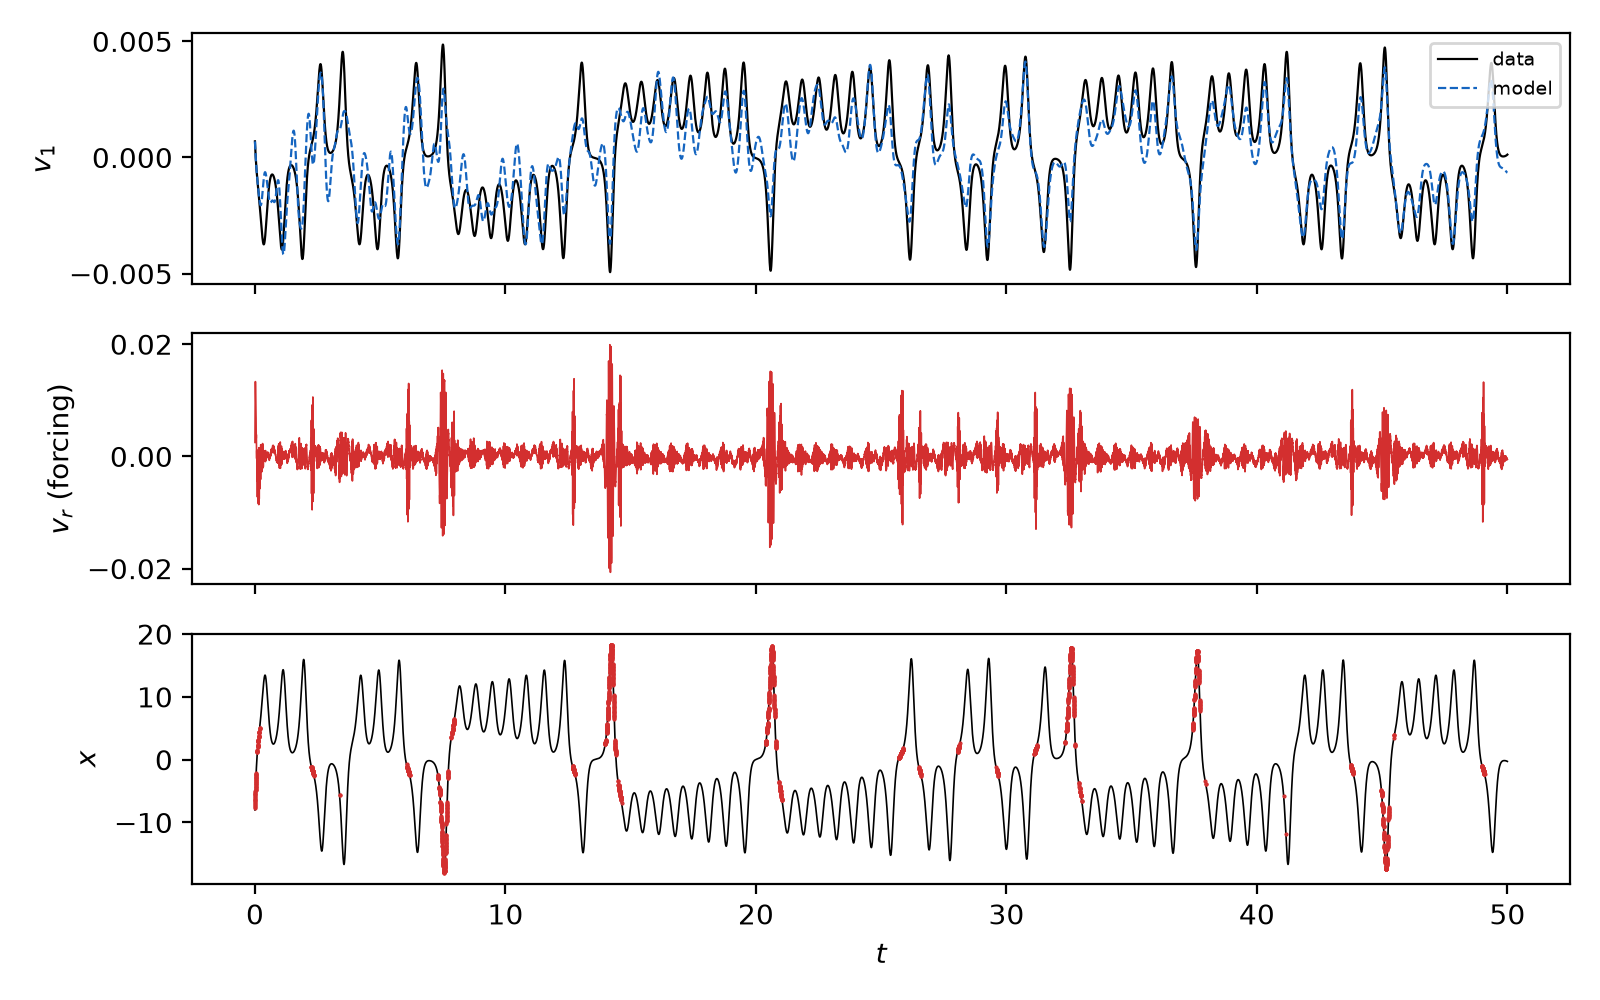
\includegraphics[width=0.78\linewidth]{figures/ch08-havok.png}\hfill
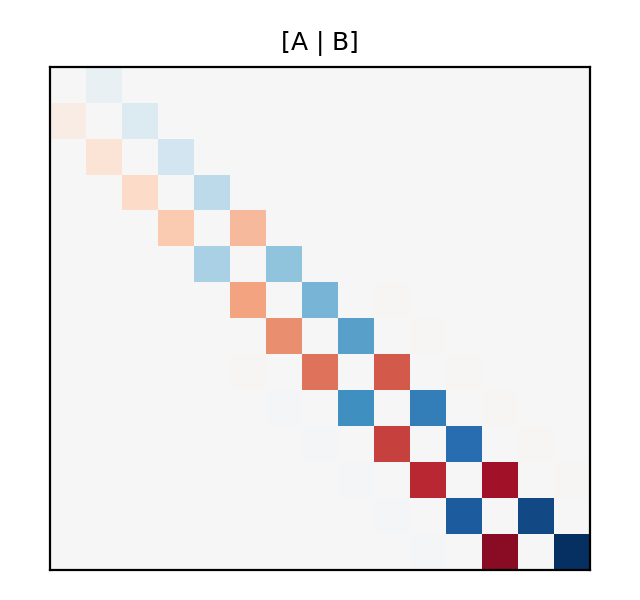
\includegraphics[width=0.2\linewidth]{figures/ch08-havok-A.png}
\caption{Output of \file{ch08_havok.py}. Top: $v_1$ from the data (black) and from the linear model \eqref{eq:hv-model} driven
by the measured forcing (blue dashed); correlation $0.92$ over 50 time units. Middle: the forcing $v_r$, quiet with intermittent
bursts. Bottom: $x(t)$, red where $v_r^2$ exceeds a threshold: the bursts sit at the lobe switches. Right: the matrix $[A\,|\,B]$,
sparse, antisymmetric, nonzero only next to the diagonal.}\label{fig:hv-lorenz}
\end{nfigure}

The script prints a relative residual of $0.97$ for the $v_r$ row, i.e.\ it is not fitted at all, against at most $0.36$ for the
other rows (and much less for the leading ones).

\paragraph{Prediction.} $v_r$ cannot be predicted, but it can be \emph{measured} in real time: project the last window of data
onto the columns of $U$ \ts{8}{1}{27:16}\ts{8}{1}{27:37}. When $v_r^2$ exceeds a threshold, colour the trajectory red: the red flag
rises before the switch, about one revolution ahead \ts{8}{1}{27:57}\ts{8}{1}{28:18}\ts{8}{1}{28:38}\ts{8}{1}{28:59}. It is ``not
perfect'', not every switch is caught \ts{8}{2}{19:23}. On the embedded attractor, white (small forcing) regions are one big
linear Koopman model surrounding the three fixed points; red regions, coherent and not random, mark where essential nonlinearity
acts \ts{8}{1}{29:19}\ts{8}{1}{29:40}\ts{8}{1}{30:01}\ts{8}{1}{30:21}. A typical sequence: four inner revolutions on the right lobe
(white), the flag goes up at point B, one more revolution, switch to the left lobe; there the forcing drops, three revolutions,
flag at D, switch back \ts{8}{1}{33:08}\ts{8}{1}{33:29}\ts{8}{1}{33:49}.

\begin{remark}[Perron--Frobenius almost-invariant sets]
The Perron--Frobenius operator, which advances densities, is dual to Koopman. Its almost-invariant sets for Lorenz are two
interleaved regions (the inner part of one lobe joined to the outer band of the other), and their outer boundaries line up with
the red regions of HAVOK: two very different analyses agree \ts{8}{1}{30:42}\ts{8}{1}{31:02}\ts{8}{1}{31:43}. That the linear part
fails somewhere is unavoidable: a finite linear model has one fixed point, Lorenz has three \ts{8}{1}{32:27}\ts{8}{1}{32:47}.
\end{remark}

% ------------------------------------------------------------------
\section{Real systems: magnetic field reversal and measles}\label{sec:hv-examples}

HAVOK has been applied to R\"ossler, the Mackey--Glass delay equation, the double pendulum, a model of Earth's magnetic field,
electrocardiogram (ECG) and sleep electroencephalogram (EEG) recordings, and measles in New York City; all the code is online
\ts{8}{1}{25:11}\ts{8}{1}{25:32}\ts{8}{1}{25:53}\ts{8}{1}{26:14}.

\begin{casestudy}[Reversals of Earth's magnetic field]
A simulation of averaged magnetohydrodynamic equations, forced by turbulent fluctuations in the Earth's interior, reproduces
geomagnetic reversals \ts{8}{1}{34:30}\ts{8}{1}{34:50}\ts{8}{3}{3:07}. The embedded attractor has two clusters, North pole up and
North pole down, with long stays and sudden jumps; reversals are recorded in the Earth's crust \ts{8}{1}{35:11}\ts{8}{1}{35:31}.
Colouring red where $v_r^2$ exceeds the threshold, the red segments are the reversals \ts{8}{1}{36:12}; there are also near-reversals
that come back \ts{8}{3}{4:10}. Zooming in: just before a flip, $v_1$ is still within its normal fluctuations, and no one could tell
by eye, but the forcing jumps ``clear as day'' \ts{8}{1}{36:53}\ts{8}{1}{37:13}\ts{8}{3}{5:52}. Not 100\%, but a real heads-up
\ts{8}{3}{6:13}.
\end{casestudy}

\begin{casestudy}[Measles in New York City]
Biweekly measles cases in New York, 1928--1964, a classic of delay embedding since Sugihara and May (Nature, 1990)
\ts{8}{1}{37:35}\ts{8}{3}{6:33}. In eigen time-delay coordinates the quiet state is the origin and each outbreak is a burst-and-return
loop; the bigger the loop, the worse the outbreak \ts{8}{1}{37:56}\ts{8}{1}{38:16}. Large outbreaks come with large forcing; the
largest outbreak has the largest forcing event \ts{8}{1}{38:36}. The method ignores small dips in the data that might have been
false alarms and waits for the real precursor \ts{8}{1}{38:57}\ts{8}{3}{7:56}; the first moments of the forcing are already larger
for the worst outbreak, hinting at a prediction of severity \ts{8}{1}{39:18}\ts{8}{3}{8:16}\ts{8}{3}{8:36}.
\end{casestudy}

\begin{history}[Sugihara and May]
George Sugihara and Robert May, \emph{Nonlinear forecasting as a way of distinguishing chaos from measurement error in time
series}, Nature 344 (1990) 734--741, used delay embeddings and nearest-neighbour forecasts on the New York measles and chickenpox
records: measles forecasts degraded with the horizon as for low-dimensional chaos, chickenpox looked like noise around a seasonal
cycle. May is the same ecologist who popularized the logistic map (\cref{sec:si-logistic}).\par
\textit{References:} the paper cited; Brunton et al., Nat.\ Commun.\ 8 (2017).
\end{history}

% ------------------------------------------------------------------
\section{The structure of the HAVOK model}\label{sec:hv-structure}

The Lorenz HAVOK matrix has a striking structure \ts{8}{1}{39:59}\ts{8}{4}{0:44}\ts{8}{4}{1:05}:
\begin{itemize}
  \item \emph{sparse}: nonzero only on the first super- and sub-diagonals \ts{8}{1}{40:20}\ts{8}{1}{41:02};
  \item \emph{antisymmetric}: entries come in equal and opposite pairs \ts{8}{4}{1:25};
  \item the signs on one off-diagonal follow a pattern: four of one sign, then one of the other, three, one, two, one, one
        \ts{8}{1}{41:22}\ts{8}{4}{3:08};
  \item the coefficients are nearly integer multiples of 5: $\pm4.9$, $\pm9.9$, $\pm15.1$, \dots\ \ts{8}{1}{41:43}\ts{8}{4}{2:27}\ts{8}{4}{2:47}.
\end{itemize}
It was discovered by applying SINDy to delay coordinates: even with nonlinear terms allowed, the most parsimonious model was this
sparse linear one, which suggested the connection to Koopman \ts{8}{1}{40:20}\ts{8}{1}{40:41}\ts{8}{4}{1:45}\ts{8}{4}{2:07}. The script
reproduces it: the super-diagonal of $A$ is $-5.18$, $-9.88$, $-13.63$, $-18.76$, $+23.25$, $-28.62$, $-33.47$, $-38.88$: multiples
of 5 (approximately) with a sign flip after the fourth.

\begin{proposition}[Antisymmetric tridiagonal structure from Legendre polynomials]\label{prop:hv-legendre}
If the delay window is short and the modes $u_k$ are (discretized, normalized) Legendre polynomials $P_{k-1}$ on the window, then
the derivative operator in this basis is approximately tridiagonal and antisymmetric, with entries growing linearly with $k$.
\end{proposition}
\begin{proof}[Sketch]
Write $x(t+s)=\sum_kv_k(t)u_k(s)$ for $s$ in the window; then $\dot v_k=\langle u_k,\partial_s x\rangle$, so $A$ is the matrix of
$\partial_s$ in the Legendre basis, truncated. The recurrence $(2n+1)P_n=P_{n+1}'-P_{n-1}'$ makes $\langle P_m,P_n'\rangle$ vanish
unless $m<n$ with $m+n$ odd; a sliding window (data moving through it) symmetrizes this into the antisymmetric part, and the
coefficients scale like $n/\text{window length}$, with nearest neighbours dominating. A precise derivation is in the
literature on HAVOK and on the ``Legendre memory'' of delay embeddings.
\end{proof}

\paragraph{Polynomial modes.} The eigen time series that matter, the columns of $U$, are polynomials for almost all examples:
constant, linear, parabola, cubic, \dots\ \ts{8}{1}{42:25}\ts{8}{1}{42:45}. Convolving a short sliding window of data with this
basis gives the current $v_1,\dots,v_{r-1}$ and the forcing $v_r$ (the 15th, in red) \ts{8}{1}{42:04}\ts{8}{1}{43:05}.

\paragraph{The integer model.} Brunton built a ``neighbouring'' system by hand with exactly this pattern and coefficients
$5,10,15,20,-25,30,35,40,-45,\dots$, and drove it with the $v_{15}$ measured from the real Lorenz system: it shadows the Lorenz
dynamics, lobe switching included, not perfectly but far better than expected; nobody knows why
\ts{8}{1}{43:46}\ts{8}{1}{44:07}\ts{8}{1}{44:27}\ts{8}{1}{44:48}\ts{8}{4}{3:50}\ts{8}{4}{4:32}.

\paragraph{The general lesson.} From data to dynamics \ts{8}{1}{45:09}\ts{8}{1}{45:30}\ts{8}{2}{21:46}:
\begin{enumerate}
  \item measure the right things (embedding theory and observability tell what is a good measurement);
  \item find a representation in which the dynamics is simple: for chaotic systems, eigen time-delay coordinates, a Koopman
        invariant basis in which the dynamics is linear over most of phase space;
  \item regression is the easy part.
\end{enumerate}
Where the forcing is active the system is genuinely nonlinear, but those are exactly the interesting regions: lobe switches,
reversals, outbreaks \ts{8}{1}{46:10}\ts{8}{1}{46:31}.

\begin{keyformulas}
\begin{itemize}
  \item Hankel matrix of $x(t)$ $=$ Krylov sequence $x,\K x,\K^2x,\dots$; $H=U\Sigma V^*$; low rank $\Rightarrow$ leading $u_k$ span an
        approximately Koopman-invariant subspace.
  \item HAVOK: $\dot{\vb v}_{1:r-1}=A\vb v_{1:r-1}+Bv_r$; $v_r$ intermittent, heavy-tailed, active before lobe switches.
  \item $A$: sparse, tridiagonal, antisymmetric, entries $\approx$ multiples of 5 for Lorenz; modes $\approx$ Legendre polynomials.
\end{itemize}
\end{keyformulas}

\section*{Exercises}

\begin{exercise}[Choice of $q$ and $r$]
Run \file{ch08_havok.py} with $q=50,100,200$ and $r=11,15,21$. How do the singular values, the fit residuals and the correlation of
the model change? Use the Gavish--Donoho optimal hard threshold ($\approx2.858\,\sigma_{\text{med}}$ for a square-ish matrix with
unknown noise; for a $q\times m$ matrix use their formula $\omega(\beta)$) to pick $r$ objectively.
\end{exercise}

\begin{exercise}[A bad measurement]
Repeat the analysis with $z(t)$ instead of $x(t)$. Explain, using the symmetry $(x,y,z)\mapsto(-x,-y,z)$, why the embedded attractor
cannot be diffeomorphic to Lorenz and what happens to the forcing.
\end{exercise}

\begin{exercise}[Precursor statistics]
Using the script, define switches as sign changes of $x$ that persist, and red-flag events as upward crossings of the threshold by
$v_r^2$. Compute the fraction of switches preceded by a flag within one revolution and the false-alarm rate, as functions of the
threshold. Remember that $v_r(t_i)$ uses the window $[t_i,t_i+q\,dt]$: shift it to make the forecast causal.
\end{exercise}

\begin{exercise}[Legendre basis]
Plot the first six columns of $U$ against $s\in[0,q\,dt]$ and compare them with the Legendre polynomials $P_0,\dots,P_5$ mapped to the
window. Compute $\langle u_m,\partial_su_n\rangle$ numerically and compare with $A$.
\end{exercise}

\begin{exercise}[Integer model]
Build the antisymmetric tridiagonal matrix with super-diagonal $-5,-10,-15,-20,25,-30,\dots$ (signs as in the script) and drive it with
the measured $v_r$. Compare its $v_1$ with the data and with the fitted HAVOK model.
\end{exercise}

\end{paracol}
